\chapter{Charged pion reconstruction and identification}
\label{ch:reconstruction}
\graphicspath{{Chapter-Reconstruction/figures/}}

Charged particles produced in collisions at the ATLAS \ac{IP} travel helical paths through the \id due to the solenoid magnetic field.
The three subdetectors register hits at various space-point locations as each of these particles passes through them, often 11 silicon and 15--30 \trt hits for a typical particle of sufficiently high \pt.
The trajectories of these particles must be reconstructed from the collection of all the space-point hits in order to infer the initial momentum of all of the collision products.
This procedure is non-trivial and computationally intensive, particularly because charged particles lose energy and may be scattered where they pass through detector elements.

\section{Tracking algorithm}

%% for general track fitting overview see:
%% http://www.phys.ufl.edu/~avery/fitting.html

%% Kalman filter -- dedicated subsection?

\cite{Aad:2010bx} %% ID commissioning and calibration - good summary (already referenced -- not as much detail in track alg)
\cite{Cornelissen:2007vba} %% ATLAS new tracking (NEWT)
\cite{Cornelissen:2008zza} %% global chi^2 track fitter

\section{Track reconstruction performance}

\begin{figure}[t]
  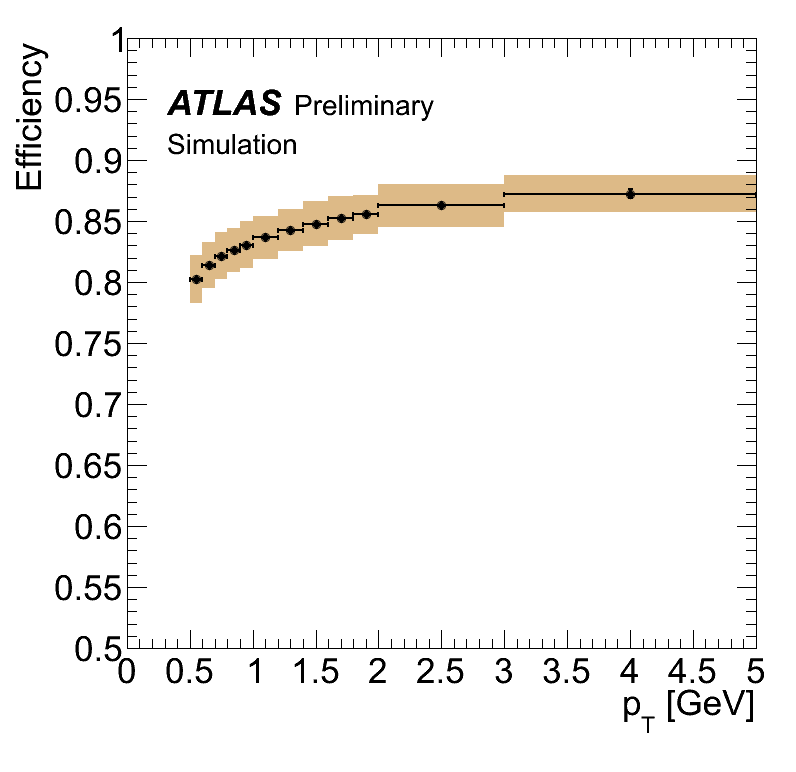
\includegraphics[width=0.49\linewidth]{atl_com_phys_2012_1541_fig_07_eff_pt.png}
  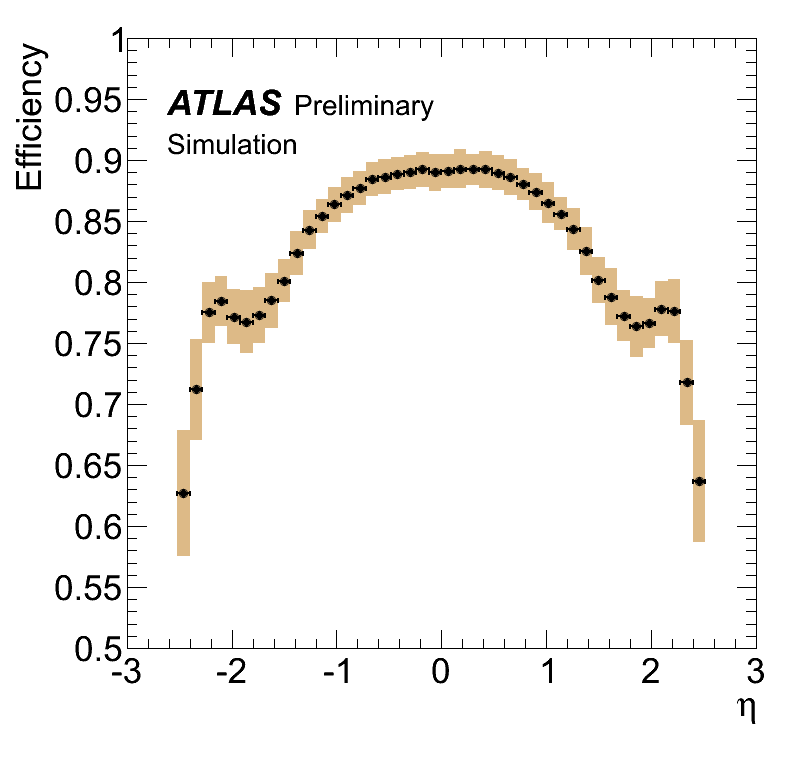
\includegraphics[width=0.49\linewidth]{atl_com_phys_2012_1541_fig_08_eff_eta.png}
  \caption{The Run-1 track reconstruction efficiency as a function of transverse momentum (left) and pseudorapidity (right).}
  \label{fig:trk_eff}
\end{figure}

\section{Pion identification}


